\documentclass[10pt]{exam}
\usepackage[phy]{template-for-exam}
\usepackage{multirow}
\usepackage[table,dvipsnames]{xcolor}
\usepackage{pgf-pie}
\usepackage{wrapfig}
\usepackage{enumitem}
\usepackage{graphicx}
\graphicspath{{./images}}
\setlist[enumerate]{topsep=0pt,itemsep=-1ex,partopsep=1ex,parsep=1ex}
\usepackage[super]{nth}


\newcommand{\mg}{\rowcolor{Goldenrod}}


\title{Course Information Guide \\ Physics I}
\author{Rohrbach}


\begin{document}

\maketitle

\noindent Mr. Rohrbach
%
\hfill
%
(317) 544-5000
%
\hfill
%
\texttt{ZJRohrbach@avon-schools.org}

\vspace{-0.5em}


\section*{Course Description}

Physics is the study of how the universe works on the most fundamental level.  In this 
class, you will use your powers of observation and logical as well as mathematical 
reasoning to describe, explain, and predict the behavior of objects.

\paragraph{Course Goals} 
As a result of taking Physics I, you will:

\begin{enumerate}
	\item Know and understand the process that is used to make the scientific discoveries that 
				are reported in the media or in the workplace
	\item Understand the scientific principles that underlie motion, forces, waves, and electricity.
	\item Apply your mathematical skills to solving real-world problems
	\item Develop problem solving and scientific literacy skills
\end{enumerate}

\section*{Required Materials}

You are expected to bring the following materials with you to class every day.
%
\begin{center}

	\vspace{-0.5em}

	\begin{tikzpicture}
		
		
		\node at (0, -1) {\small Notebook};
		\node at (0, -1.3) {\footnotesize \it (will be provided)};
		\node at (0,0) {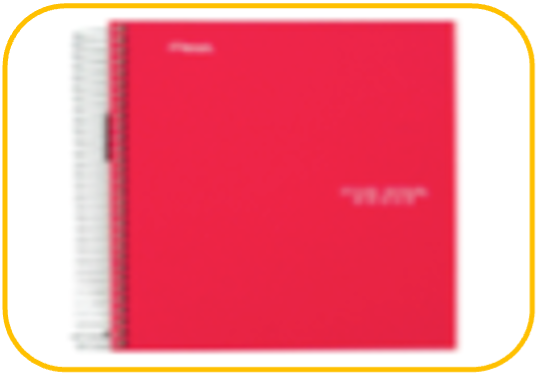
\includegraphics[width=2.4cm]{notebook}};


		\node at (3, -1) {\small Reading Book};
		\node at (3, -1.3) {\footnotesize \it (from school library)};
		\node at (3,0) {
\includegraphics[width=2.4cm]{book}};


		\node at (6, -1)  {\small Laptop};
		\node at (6,0) {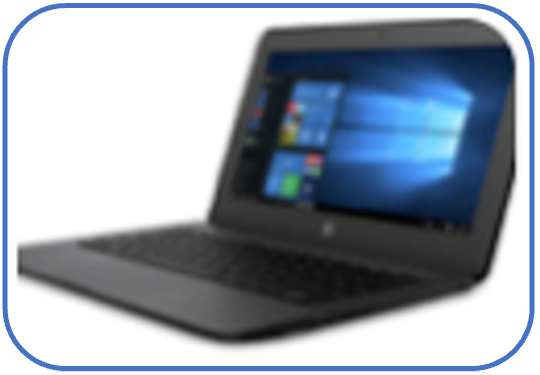
\includegraphics[width=2.4cm]{laptop}};

		
		\node at (9, -1)  {\small Computer Charger};
		\node at (9,0) {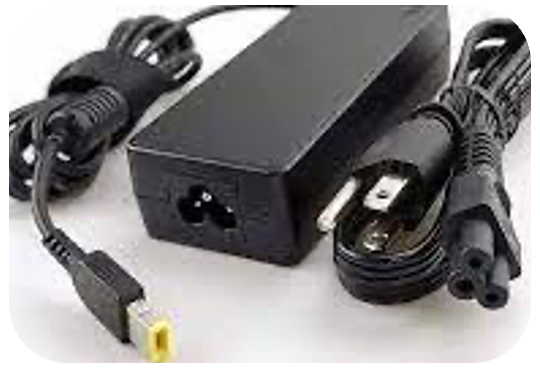
\includegraphics[width=2.4cm]{charger}};
		

	\end{tikzpicture}

\end{center}
%
Additionally, please purchase and bring the following items into the classroom for communal use by Friday, August 9:
%
\begin{center}

	\vspace{-0.5em}

	\begin{tikzpicture}[x=0.8cm,y=1.2cm]
		
		
		\node[rectangle,text width=6cm,anchor=north,align=center] at (0, -1) {\small one four-pack of disposable clear tape dispensers};
		\node at (0,0) {
\includegraphics[width=2.4cm]{tape}};

		\node[rectangle,text width=6cm,anchor=north,align=center] at (8, -1) {\small one tissue box};
		\node at (8,0) {
\includegraphics[width=2.4cm]{tissues}};

		

	\end{tikzpicture}

\end{center}


\section*{Methods of Evaluation}

\begin{minipage}{4.4in}
Your pre-exam grade will be based on the methods of 
evaluation shown to the right. The weighting of each of these categories is subject to change. Your overall class grade will consist of the pre-exam grade (85\%) and the final exam grade (15\%).

\indent

Tests may be corrected for half credit back on missed 
questions.  Test corrections are due by midterm.  In other words, test corrections for units completed before the midterm will not be accepted after the midterm.  Directions on how to do corrections will be given later.
\end{minipage}
%
\begin{minipage}{2in}
	\begin{flushright}
		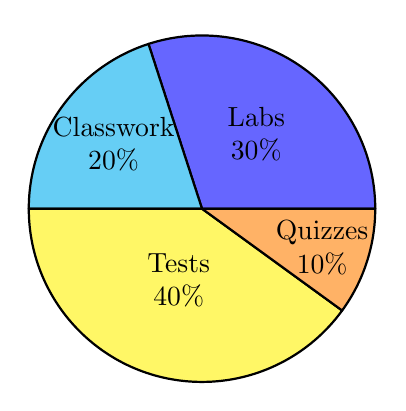
\begin{tikzpicture}
			\pie[text=inside, radius=2.2]{
				30/Labs,
				20/Classwork,
				40/Tests,
				10/Quizzes
			}
		\end{tikzpicture}
	\end{flushright}
\end{minipage}


\section*{Classroom Expectations}

\begin{center}
  \begin{tabular}
    {
      p{.15\textwidth}
      p{.03\textwidth}
      p{.7\textwidth}
		}
		
    \hline
      \mg \bf Accountable 
      			&  1. & Start the period with your {\bf calculator}, 
                  {\bf notebook}, and {\bf reading book} on your 
                  desk.
      \\
      \mg   &  2. & Bring your {\bf computer} and {\bf charger} with you
                  every day.
      \\
      \mg 	&  3. & Try to take care of restroom breaks 	
									outside of class.
      \\
     	\mg   &  4. & Be in the classroom by the time the bell 
                  rings.
                  \vspace{-1em}
                  \begin{quotation}
                  	\noindent\small
										\textit{My tardy policy is the same as the policy listed on p. 12  of the AHS Student Handbook.  You are tardy if you are not in the classroom by the time the bell rings.  You will be given a detention on your \nth{3} and \nth{4} tardies and referred to Saturday School for \nth{5} and \nth{6} tardies.}
                  \end{quotation}
      \\  
    
    \hline
    \bf Respectful
          &  5. & SSR time is for silent reading.
                 	\vspace{-1em}
                  \begin{quotation}
                  	\noindent\small
										\textit{We will have 10 minutes of sustained silent reading (SSR) 
										at the beginning of the period.  Why do we do silent reading in a 
										science class?  Research shows that people who read do better in 
										school and have lower levels of stress.  It also is an opportunity to 
										take a breath and set the tone for the class period.}
                  \end{quotation}
          \\   
          &  6. & Quietly listen to the speaker.         
          \\  

    \hline
      \mg \bf Engaged
      		&  7. & Keep phones and earbuds put away.
                  \vspace{-1em}
                  \begin{quotation}
                  	\noindent\small
										\textit{In Physics class, there is no instructional need for cell phones or earbuds.  They should therefore be put away at all times.  Failure to comply will result in the progressive discipline outlined in the AHS Student Handbook on p. 25.}
                  \end{quotation}
      \\
      \mg &  8. & When you are finished with your work, 
                  you may read a book.
      \\
      \mg &  9. & Stay engaged and working until the 
                  {\bf two-minute alarm}.
      \\
      \mg & 10. & Persevere through difficult problems.
      \\  

    \hline
  \end{tabular}
\end{center}


\section*{Other Class Policies}

\paragraph{Late Work}
	Deadlines for assignments will be announced in class and posted on Schoology.  Late work is subject to a 50\% penalty.  Late work for a particular unit will not be accepted after the test is given for that unit.

\paragraph{Absences and Makeup Work}
	If you are absent, it is your responsibility to check Schoology for your required makeup work and contact Mr. Rohrbach with any questions.  Required makeup work is due in a timely manner.  	Mr. Rohrbach will often also post additional video explanations and recordings on Schoology for students who are absent. You should plan to watch these recordings and take notes over them before you return to school.

	There are some ``nonessential assignments'' that we do in class which will not need to be made up.  Students with \emph{excused} absences will be exempted from these assignments in the grade book.  Students with \emph{unexcused} or \emph{unverified} absences will receive a zero, which cannot be made up.  This is in line with the policy in the AHS Student Handbook on p. 14.

	\begin{center}
		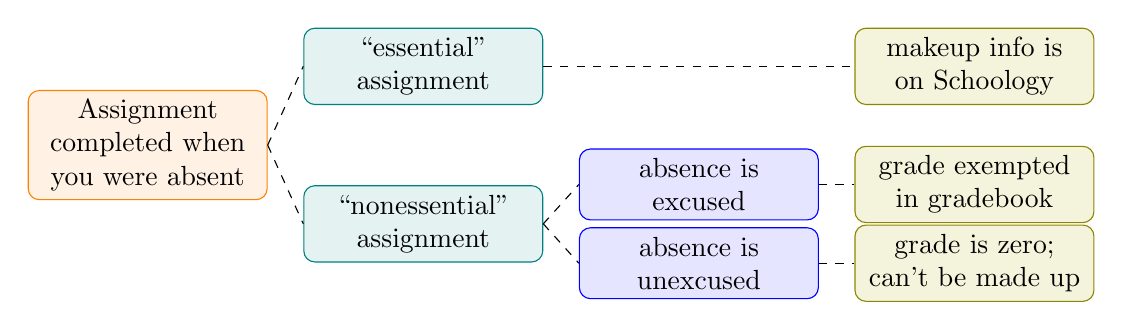
\begin{tikzpicture}[every node/.style = {
				draw,
				rectangle,
				rounded corners,
				text width=2.8cm,
				text centered
			},
			arrow/.style = {
				dashed
			},
			levela/.style = {orange,fill=orange!10,text=black},
			levelb/.style = {teal,fill=teal!10,text=black},
			levelc/.style = {blue,fill=blue!10,text=black},
			leveld/.style = {olive,fill=olive!10,text=black},
			x=3.5cm, y=0.5cm
			]
			\node[levela] (assmt) 
				{Assignment completed when you were absent};
	
			\node[levelb] at (1,2) (essential) 	
				{``essential'' assignment};
			\node[levelb] at (1,-2) (nonessential) 	
				{``nonessential'' assignment};
	
			\node[levelc] at (2,-3) (unexcused) 	
				{absence is unexcused};
			\node[levelc] at (2,-1) (excused) 	
				{absence is excused};
	
			\node[leveld] at (3,2) (schoology) 	
				{makeup info is on Schoology};
			\node[leveld] at (3,-1) (exempt) 	
				{grade exempted in gradebook};
			\node[leveld] at (3,-3) (zero) 	
				{grade is zero; can't be made up};
	
			\draw[arrow] (assmt.east) -- (nonessential.west);
			\draw[arrow] (assmt.east) -- (essential.west);
			\draw[arrow] (essential.east) -- (schoology.west);
			\draw[arrow] (nonessential.east) -- (unexcused.west);
			\draw[arrow] (nonessential.east) -- (excused.west);
			\draw[arrow] (excused.east) -- (exempt.west);
			\draw[arrow] (unexcused.east) -- (zero.west);
	
		\end{tikzpicture}
	\end{center}

\paragraph{Contacting Mr. Rohrbach}
	Parents and students should feel free to contact Mr Rohrbach at any time via email (\texttt{ZJRohrbach@avon-schools.org}), phone (317-544-5000 x5131), \mbox{ParentSquare}, or Schoology.




\end{document}